\subsection*{Общая характеристика работы}

\newcommand{\actuality}{\underline{\textbf{Актуальность темы.}}}
\newcommand{\aim}{\underline{\textbf{Целью}}}
\newcommand{\tasks}{\underline{\textbf{задачи}}}
\newcommand{\defpositions}{\underline{\textbf{Основные положения, выносимые на~защиту:}}}
\newcommand{\novelty}{\underline{\textbf{Научная новизна:}}}
\newcommand{\influence}{\underline{\textbf{Практическая значимость}}}
\newcommand{\reliability}{\underline{\textbf{Достоверность}}}
\newcommand{\probation}{\underline{\textbf{Апробация работы.}}}
\newcommand{\contribution}{\underline{\textbf{Личный вклад.}}}
\newcommand{\publications}{\underline{\textbf{Публикации.}}}


{\aim} работы является разработка интеллектуальной системы повышения эффективности деятельности ИТ-службы предприятия. \par
{\scope}~--- разработка методов и алгоритмов решения задач системного анализа, оптимизации, управления, принятия решений и обработки информации в ИТ-отрасли.\par
{\subject}  является процесс регистрации и устранения проблемных ситуаций, возникающих в ИТ-инфраструктуре предприятия.\par

Для достижения поставленной цели необходимо было решить следующие {\tasks}:
\begin{enumerate}
  \item Провести теоретико-множественный и теоретико-информационный анализ сложных систем в области поддержки информационной инфраструктуры;
  \item Создать модель целевой области;
  \item Исследовать модели мышления и выбрать наиболее подходящую;
  \item На основе выбранной модели мышления разработать модель проблемно-ориентированной системы управления, принятия решений и оптимизации процесса принятия, анализа и обработки запросов пользователя в области обслуживания информационной структуры предприятия;
  \item Создать архитектуру приложения на основе модели;
  \item Реализовать на основе этой архитектуры прототип интеллектуальной вопросно-ответной системы повышения эффективности деятельности ИТ-службы предприятия;
  \item Провести апробацию прототипа на тестовых данных.
\end{enumerate}

\defpositions
\begin{enumerate}
  \item Теоретико-множественный и теоретико-информационный анализ сложных систем в области поддержки информационной инфраструктуры;
  \item Построенная модель проблемно-ориентированной системы управления, принятия решений и оптимизации технических объектов в области обслуживания информационной инфраструктуры;
  \item Созданный прототип программной реализации модели проблемно-ориентированной системы управления, принятия решений и оптимизации обработки запросов пользователя в области обслуживания информационной инфраструктуры;
  \item Апробация прототипа проблемно-ориентированной системы управления, принятия решений и оптимизации деятельности на контрольных примерах и анализ ее результатов.
\end{enumerate}

\novelty проведенного исследования состоит в следующем:
\begin{enumerate}
  \item Создана модель проблемно-ориентированной системы управления, принятия решений в области обслуживания информационной структуры предприятия на основе модели мышления;
  \item Представлены новая модель данных для модели мышления и оригинальный способ хранения для этой модели, эффективный по сравнению с другими базами данных;
  \item Выполнено оригинальное исследование моделей мышления применительно к области обслуживания информационной структуры предприятия;
  \item На основе модели мышления Мински созданы архитектура системы обслуживания информационной структуры предприятия и программный прототип этой системы.
\end{enumerate}

\influence\ 
Система, разработанная в рамках данной диссертации носит значимый практический характер. Идея работы зародилась под влиянием производственных проблем в ИТ-отрасли, с которыми автор сталкивался каждый день в процессе разрешения различных инцидентов, возникающих в деятельности службы технической поддержки \icl~--- одном из крупнейших системообразующих предприятий ИТ-области Республике Татарстан. Поэтому было необходимо выработать глубокое понимание конкретной предметной области, чтобы выбрать приемлемое решение, получившее практическое применение в работе на проекте поддержки крупной сети продуктовых магазинов. \par
\reliability\ научных исследований и практических рекомендаций
базируется на корректной постановке общих и частных рассматриваемых задач,  использовании известных фундаментальных теоретических положений системного анализа, достаточном объёме данных, использованных при статистическом моделировании, и широком экспериментальном материале, использованном для численных оценок достижимых качественных показателей. \par 
Исследования, проведенные в диссертации, соответствуют паспорту специальности 05.13.01~--- Системный анализ, управление и обработка информации, сопоставление приведено в таблице \ref{ResearchDescription}.

\begin{longtable}{|p{7cm}|p{9cm}|}
 \caption[Сопоставление направлений исследований в рамках специальности 05.13.01 и исследований, проведенных в диссертации]{Сопоставление направлений исследований в рамках специальности 05.13.01 и исследований, проведенных в диссертации}\label{ResearchDescription} \\ 
 \hline
 
 \multicolumn{1}{|c|}{\textbf{Направление исследования}} & \multicolumn{1}{c|}{\textbf{Результат работы}}  \\ \hline 
\endfirsthead
\multicolumn{2}{c}%
{{\bfseries \tablename\ \thetable{} -- продолжение}} \\
\hline \multicolumn{1}{|c|}{\textbf{Направление исследования}} &
\multicolumn{1}{c|}{\textbf{Результат работы}}  \\ \hline 
\endhead

\hline \multicolumn{2}{|r|}{{Продолжение следует}} \\ \hline
\endfoot

\hline \hline
\endlastfoot
\hline
   Разработка критериев и моделей описания и оценки эффективности решения задач системного анализа, оптимизации, управления, принятия решений и обработки информации & В рамках работы была разработана модель системы принятия решения и обработки информации в области решения запросов пользователя на естественном языке. \\
   \hline
   Разработка проблемно-ориентированных систем управления, принятия решений и оптимизации технических объектов & По модели, разработанной в предыдущем пункте был разработан прототип системы принятия решения Thinking Understanding, который был испытан на модельных данных.\\
   \hline
   Методы получения, анализа и обработки экспертной информации & В рамках системы TU был разработан метод обработки экспертной информации - обучение при помощи модели мышления TU, основанной на принципах модели 6-ти Марвина Мински. \\
   \hline
   Разработка специального математического и алгоритмического обеспечения систем анализа, оптимизации, управления, принятия решений и обработки информации & В рамках разработки системы TU были созданы специальные алгоритмы для анализа запросов пользователя и принятия решений.\\
  \hline 
  Теоретико-множественный и теоретико-информационный анализ сложных систем & В рамках работы был проведен комплексный анализ области поддержки программного обеспечения, с помощью которого была построена система данной области и выделены участки для оптимизации принятия решений.\\
  \hline
  Методы и алгоритмы интеллектуальной поддержки при принятии управленческих решений в технических системах & Система, разработанная в рамках данной работы в включает в себя инновационные методы и алгоритмы поддержки принятия решений, использующих в своей основе модель мышления на базе модели мышления Человека, описанной в книге Марвина Мински. \\ 
  \hline
  Визуализация, трансформация и анализ информации на основе компьютерных методов обработки информации & Представлена наглядная визуализация данных по системному анализу области удаленной поддержки инфраструктуры. \\
  \hline	
\end{longtable}


\probation\
 Основные результаты диссертационной работы докладывались на следующих конференциях:
\begin{itemize}
	\item Десятая молодежная научная школа-конференция "Лобачевские чтения~---2011. Казань, 31 октября~--4 ноября 2011";
	\item 3rd World Conference on Information Technology (WCIT-2012); 
	\item Искусственный интеллект и естественный язык (AINL-2013);
	\item Электронная Казань~--- 2014;
	\item Электронные библиотеки: перспективные методы и технологии, электронные коллекции (RCDL-2014);
	\item Agents and multi-agent systems: technologies and applications (AMSTA-2015).
\end{itemize}
Практическая апробация результатов работы проводилась на выгрузке инцидентов из системы регистрации запросов службы технической поддержки ИТ-инфраструктуры \icl. Созданная система показала требуемые результаты (процент успешно обработанных запросов более чем 30\%) обработки данной информации.
\contribution\ Автор исследовал целевую область: проводил анализ запросов пользователей и классифицировал их, вместе с Талановым Максимом Олеговичем изучал модель мышления Марвина Мински; создавал базовую архитектуру систему; вместе с Талановым Максимом Олеговичем проводил разработку компонентов модели, адаптируя теорию Марвина Мински. Автор проводил испытание системы на целевых запросах; отлаживал работу системы.
\publications\ Основные результаты по теме диссертации изложены в 9 печатных изданиях  \cite{Lobachevskii},\cite{WCIT-2012},\cite{AINL-2013},\cite{ISGZ}, \cite{IJSE-1}, \cite{IJSE-2}, \cite{RCDL-2014}, \cite{AMSTA-2015}, \cite{VAK-1}, из которых статьи \cite{RCDL-2014},\cite{AMSTA-2015} проиндексированы в БД Scopus, статья \cite{AMSTA-2015} проиндексирована в БД Web Of Science, работа \cite{VAK-1} опубликована в журнале из списка ВАК, статья  \cite{ISGZ} проиндексирована в БД РИНЦ, работы \cite{Lobachevskii},\cite{WCIT-2012},\cite{AINL-2013},\cite{ISGZ} опубликованы в материалах международных и всероссийских конференций.



 % Характеристика работы по структуре во введении и в автореферате не отличается (ГОСТ Р 7.0.11, пункты 5.3.1 и 9.2.1), потому её загружаем из одного и того же внешнего файла, предварительно задав форму выделения некоторым параметрам

%Диссертационная работа была выполнена при поддержке грантов ...

%\underline{\textbf{Объем и структура работы.}} Диссертация состоит из~введения, четырех глав, заключения и~приложения. Полный объем диссертации \textbf{ХХХ}~страниц текста с~\textbf{ХХ}~рисунками и~5~таблицами. Список литературы содержит \textbf{ХХX}~наименование.

%\newpage
\subsection*{Содержание работы}
Во \underline{\textbf{введении}} обосновывается актуальность исследований, проводимых в рамках данной диссертационной работы, дается общая характеристика работы.
\underline{\textbf{Первая глава}} посвящена постановки задачи. Проводится обзор целевой области и обосновывается возможность ее автоматизации. В главе обосновывается состав команд поддержки информационной структуры предприятия. На Диаграмме \ref{img:ITSMTeamComposition} представлен качественно процентный состав в команд с точки зрения квалификации специалистов. \\
\begin{figure} [h] 
  \center
  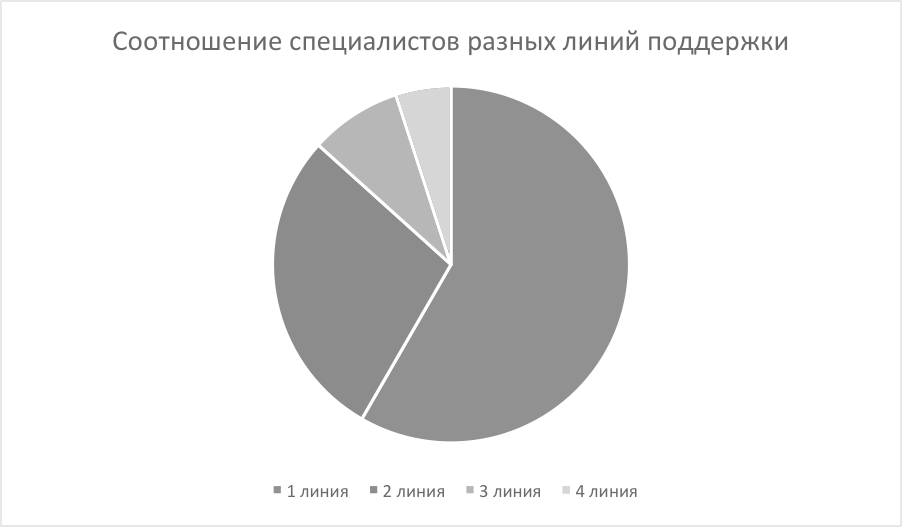
\includegraphics [scale=0.7] {ITSMTeamComposition}
  \caption{Диаграмма состава команд} 
  \label{img:ITSMTeamComposition}  
\end{figure}

В главе приведены результаты анализа категорий проблем, которые решают специалисты \ref{img:EngineerTasks}. В главе приведено технико-экономическое обоснование необходимости решения проблемы, где выведен необходимый порог в 50\% решения системой целевых инцидентов. 
\begin{figure} [h] 
  \center
  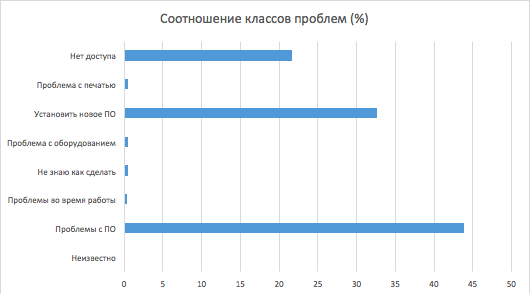
\includegraphics [scale=0.7] {EngineerTasks}
  \caption{Диаграмма соотношений типов проблем} 
  \label{img:EngineerTasks}  
\end{figure}

%=================
%===Second chapter
%=================

\clearpage
\underline{\textbf{Вторая глава}} посвящена анализу текущих решений получения, анализа и обработки экспертной информации в области обслуживания программного обеспечения и информационной инфраструктуры. Было выбрано 3 наиболее популярных на сегодняшний день решений: HPOpenView, ServiceNOW, IBMWatson. Были выработаны критерии сравнения и требования к целевой системе. В Таблице \ref{Comparsion} приведены результаты сравнения по основным критериям. В главе также был выработан набор тестовых данных, разработаны критерии оценки работы подходов обработки естественного языка, представленных в Таблице \ref{Metrics}.
\begin{table} [htbp]
  \centering
  \parbox{15cm}{\caption{Таблица метрик}\label{Metrics}}
%  \begin{center}
  \begin{tabular}{| p{5cm} ||p{5cm}|| p{5cm} |}
  \hline
  \hline
Метрика & Описание & Формула \\
  \hline
  \hline
Аккуратность	& Понимание текста обработчиком & 
$$ 
Ac=\frac{1-x}{y}
$$ где x- количество нераспознанныx слов, y количество распознанных \\
 \hline
Успешно обработанные	& Успешно обработанные инциденты & 
$$ 
P=\frac{x}{100}
$$ где x успешно обработанные \\
 \hline
Не успешно обработанные	& Неуспешно обработанные инциденты & 
$$ 
N=\frac{y}{100}
$$ где y неуспешные инциденты \\
 \hline
Результативность	& Общая результативность обработчика & 
$$ 
R=\frac{P}{N}
$$  \\
  \hline
  Общий бал	& Общая оценка обработчика & 
$$ 
T=Ac+R
$$  \\
  \hline
  \hline
  \end{tabular}
%  \end{center}
\end{table}

На основе данных критериев был проведен анализ существующих подходов, результаты которого приведены на Диаграмме \ref{img:ParserComp}. По итогам главы был сделан вывод, что наиболее эффективен подход, использующийся в комплексе OpenCog Relex.

\begin{figure} [h] 
  \center
  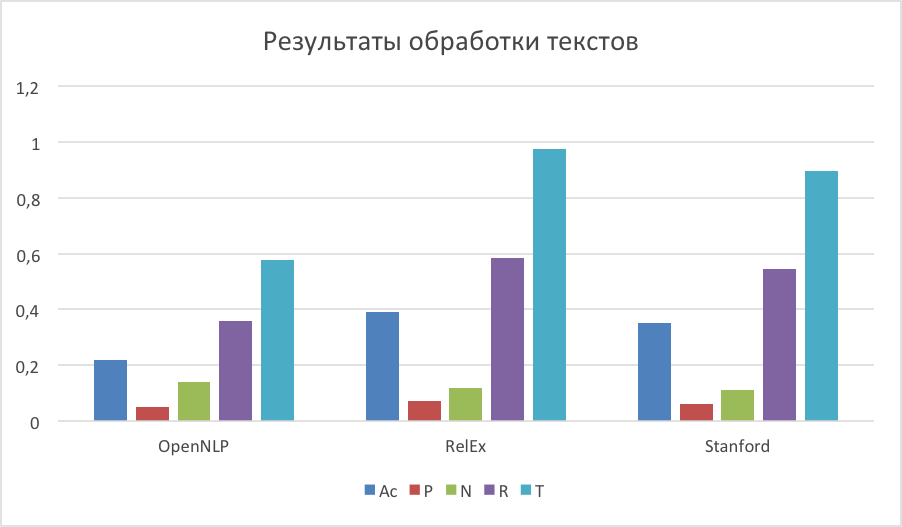
\includegraphics [scale=1.0] {ParserCompare}
  \caption{Результаты обработки текстов} 
  \label{img:ParserComp}  
\end{figure}
\clearpage


\begin{longtable}{|p{6cm}|p{0.5cm}|p{0.5cm}|p{0.5cm}|}
 \caption[Сравнительный анализ существующих решений]{Сравнительный анализ существующих решений}\label{Comparsion} \\ 
 \hline
 
 \multicolumn{1}{|c|}{\textbf{Сравнительный пункт}} & \multicolumn{1}{c|}{\textbf{HP Open View}} & \multicolumn{1}{c|}{\textbf{ServiceNOW}} & \multicolumn{1}{c|}{\textbf{IBM Watson}} \\ \hline 
\endfirsthead
\multicolumn{2}{c}%
{{\bfseries \tablename\ \thetable{} -- продолжение}} \\
\hline \multicolumn{1}{|c|}{\textbf{Сравнительный пункт}} & \multicolumn{1}{c|}{\textbf{HP Open View}} & \multicolumn{1}{c|}{\textbf{ServiceNOW}} & \multicolumn{1}{c|}{\textbf{IBM Watson}}  \\ \hline 
\endhead

\hline \multicolumn{2}{|r|}{{Продолжение следует}} \\ \hline
\endfoot

\hline \hline
\endlastfoot
\hline
   Мониторинг & Да & Да & Да \\
   \hline
   Регистрация инцидентов & Да & Да & Да\\
   \hline
   Управление системами & Да & Нет & Нет \\
   \hline 
   Создание цепи обработки (Workflow) инцидента & Да & Да & Нет \\
   \hline 
   Понимания и формализацию запросов на естественном языке & Нет & Нет & Да \\
   \hline 
   Поиск решений & Нет & Нет & Да \\
   \hline 
   Применение решений & Нет & Нет & Нет \\
   \hline
   Обучение решению инцидента & Нет & Нет & Да \\
   \hline
   Умение проводить логические рассуждения: генерализацию, специализацию, синонимичный поиск & Нет & Нет & Нет \\
   \hline
   \textbf{Итоговые очки} & 4 & 3 & 5 \\
   \hline 
\end{longtable}

\clearpage
%=================
%===Forth chapter
%=================
В \underline{\textbf{третьей главе}} приведено описание теоретического базиса системы и ее модели. Было рассмотрено четырех различных подхода и модели системы, были отмечены их плюсы и минусы. Был выбран подход на базе модели Марвина Мински и концепция уровней мышления, который являлся квинтэссенцией всех рассмотренных подходов. Он включает два главных компонента триплет Critic->Selector->WayToThink и уровни мышления. Это основные концепции, которые легли в архитектуру системы. Кроме того посредством WayToThink модель инкапсулирует результаты исследований, выполненных другими авторами в рамках других исследований и автором в рамках начальных исследований. Более подробно историю проекта можно прочитать на http://tu-project.com. 


\textbf{Критик (Critic)} представляет собой определенный триггер: внешние обстоятельства, события или иное воздействие. Например, включился свет и зрачки сузились. Обожглись и одернули руку. Критик активируется только когда для этого достаточно обстоятельств. Одновременно могут активироваться несколько критиков. Например, человек решает сложную задачу. Идет активация множество критиков: считать, технические детали, кроме того параллельно может активироваться критик переработки, сообщающей о необходимости отдыха.\\
\textbf{Селектор (Selector)} занимается выбором определенных ресурсов, которыми также являются Пути мышления. \\
\textbf{Путь мышления (WayToThink)} это способ решения проблемы. Путь мышления также может активировать следующий критик. \\

На рисунке \ref{img:csw_ex} представления расширенная модель работы триплета Критик-Селектор-Путь мышления. Критик активирует селектор, который активирует путь мышления (синий круг). Путь мышления в свою очередь может активировать критик или же совершить определенные действия. Например, зажегся зеленый свет светофора, значит можно переходить дорогу. \\
Если активировалось много критиков, значит проблему нужно уточнить, так как степень неопределенности слишком высока. Если проблема очень похожа, то можно судить по аналогии.
\begin{figure} [h] 
  \center
  \includegraphics [scale=1.0] {CSW_EX}
  \caption{Критик-Селектор-Путь мышления в разрезе ресурсов} 
  \label{img:csw_ex}  
\end{figure}
В Таблице \ref{ThinkingLevelDescription} представлено описание уровней мышления.
\begin{table} [htbp]
  \centering
  \parbox{15cm}{\caption{Описание уровней мышления Марвина Мински}\label{ThinkingLevelDescription}}
%  \begin{center}
  \begin{tabular}{| p{5cm} | p{11cm} |}
  \hline
  \hline
Уровень & Описание \\
  \hline
    \hline

Инстинктивный уровень	& На данном уровне происходят инстинктивные реакции (врожденные). Например, боязнь обжечься. Не прыгать под машину. Общую формулу для этого уровня можно выразить как "Если ..., то сделать так". \\
  \hline

Уровень обученных реакций  & На  данной уровне происходит мышление обученных реакций, то есть тех реакций, которыми человек обучается в течение жизни. Например, переходить дорогу на зеленых свет. Общую формулу для этого уровня можно выразить как "Если ..., то сделать так". \\
  \hline

Уровень рассуждений & а  данной уровне происходит мышление с использованием рассуждений. Если я сделаю так, то будет ... Например, если перебежать дорогу на зеленый свет, то можно успеть вовремя. На данном уровне сравниваются последствия нескольких решений и выбирается оптимальное. Общую формулу для этого уровня можно выразить как "Если ..., то сделать так, тогда будет так". \\
  \hline

Рефлексивный уровень  & На данном уровне происходит рассуждение с учетом анализа прошлых событий. Например, прошлый раз я побежал на моргающий зеленый и чуть не попал под машину. \\

  \hline
  Саморефлексивный уровень & На данном уровне происходит оценка себя. Строится определенная модель с помощью которой идет оценка своих поступков. Например, мое решение не пойти на это собрание было неверным, так как я упустил столько возможностей, я был легкомысленный. \\
  \hline
  Самосознательный уровень & Самозонательный уровень на данный момент характерен только для человека. На данном уровне идет оценка поступков человека с точки зрения высших идеалов и внешних оценок. Например, а что подумают мои друзья? А как бы поступил мой герой? \\
  \hline
  
  \end{tabular}
%  \end{center}
\end{table}
\clearpage
%=================
%===Fifth chapter
%=================
В \underline{\textbf{Главе 4}} приведены основные результаты работы, которые заключаются в следующем:
\begin{itemize}
	\item Теоретико-множественный и теоретико-информационный анализ сложных систем в области поддержки информационной инфраструктуры
	\item Проблемно-ориентированная система управления, принятия решений и
оптимизации технических объектов в области обслуживания IT
	\item Архитектура системы, ее реализация и испытания на модельных данных
	\item Описание компонентов системы
\end{itemize}
Архитектура системы представляет собой модульную систему. Основными компоненты системы описаны в Таблице \ref{MainComponents}. Система может функционировать в режиме обучения и в режиме решения запросов. 
\begin{longtable}{|p{7cm}|p{8cm}|}
 \caption[Основные компоненты системы ThinkingUnderstanding]{Основные компоненты системы ThinkingUnderstanding}\label{MainComponents} \\ 
 \hline
 
 \multicolumn{1}{|c|}{\textbf{Компонент}} & \multicolumn{1}{c|}{\textbf{Описание}}  \\ \hline 
\endfirsthead
\multicolumn{2}{c}%
{{\bfseries \tablename\ \thetable{} -- продолжение}} \\
\hline \multicolumn{1}{|c|}{\textbf{Компонент}} &
\multicolumn{1}{c|}{\textbf{Описание}}  \\ \hline 
\endhead

\hline \multicolumn{2}{|r|}{{Продолжение следует}} \\ \hline
\endfoot

\hline \hline
\endlastfoot
\hline
   TU Webservice & Основной компонент взаимодействия со внешними система, включая пользователя. \\
   \hline
   CoreService & Ядро системы, содержит основные классы.\\
   \hline
   DataService & Компонент работы с данными. \\
   \hline 
   Reasoner & Компонент вероятностной логики. \\
   \hline 
   ClientAgent & Компонент выполнения скриптов на целевой машине. \\
   \hline 
   MessageBus & Шина данных для системы. \\
   \hline 
\end{longtable}
В главе приводятся основной поток работы приложения.
 \begin{enumerate}
	\item Поступает запрос от пользователя \\
	User had received wrong application.
User has ordered Wordfinder Business Economical.
However she received wrong version, she received Wordfinder Tehcnical instead of Business Economical. Please assist.
	\item GoalManger устанавливает цель системы HelpUser
	\item Активируется набор Critic, привязанный к данной цели
	\item PreliminaryAnnorator разбирает фразу
	\item KnowledgeBaseAnnotator создает семантическую сеть и ссылки на нее
	\item Critic на Рефликсивном уровне запускает WayToThink ProblemSolving с целью: ResolveIncident
	\item Critic на Рефликсивном уровне выбирает WayToThink KnowingHow
	\begin{enumerate}
	\item Запускаются параллельно все Critic, которые привязаны к IncidentClassification Critic, который привязан к ResolveIncident цели, в данном случае это DirectInstruction, ProblemWithDesiredState, ProblemWithoutDesiredState \ref{ThinkingLifeCycle}
	\item Selector выбирает наиболее вероятный результат работы среди всех результатов компонентов. В данном случае будет результат работы Problem Description with desired state.
	\item KnowingHow сохраняет варианты выбора Selector.
	\item Simulation WayToThink с параметрами Создать модель текущий ситуации создает модель CurrentSituation. User, Software
	\item Reformulation WayToThink, используя результаты предыдущего шага синтезирует артефакты, которых не хватает, чтобы получить CurrentState и DesiredState. DesiredState не указан явно. WayToThink запускает Critic размышления, чтобы найти корень проблемы. Critic размышления находит CurrentState- Wordfinder Tehcnical, DesiredState-Wordfinder Business Economical
	\item Рефлексивные Critic оценивают состояние системы - на каком шаге она находится, и если цель не достигнута, то запускают другой WayToThink, который был возвращен, например, DirectInstruction. 
	\item Critic генерации решения запускает KnowingHow \ref{AppendixDHowTo} WayToThink, ExtensiveSearch.
	\item Selector выбирает наиболее вероятный путь мышления. В данном случае ExtensiveSearch, который будет находить решения, позволяющие привести систему в необходимое состояние (DesiredState). Если он не сможет, то он иницирует коммуникацию с пользователем. 
 \end{enumerate}
	 \item Рефлексивный Critic проверяет состояние системы. Если Цель достигнута, то пользователю посылается ответ.
	 \item Само Сознательные Critic активируется на данном шаге и сохраняют информацию о затратах на решение.

\end{enumerate}
В главе представлены методика и результаты верификации работы.
%=================
%===Conclusion
%=================
В \underline{\textbf{заключении}} приведены основные выводы по работе, которые заключаются в следующем:
%% Согласно ГОСТ Р 7.0.11-2011:
%% 5.3.3 В заключении диссертации излагают итоги выполненного исследования, рекомендации, перспективы дальнейшей разработки темы.
%% 9.2.3 В заключении автореферата диссертации излагают итоги данного исследования, рекомендации и перспективы дальнейшей разработки темы.

Решены следующие задачи и достигнуты следующие результаты.
\begin{enumerate}
  \item Создана модель проблемно-ориентированной системы управления, принятия решений в области обслуживания информационной структуры предприятия на основе модели мышления;
  \item Представлены новая модель данных для модели мышления и оригинальный способ ее хранения, эффективный по сравнению с другими базами данных;
  \item Выполнено оригинальное исследование моделей мышления в области обслуживания информационной структуры предприятия;
  \item На основе модели созданы архитектура системы и ее прототип; 
  \item Созданы специальные алгоритмы для анализа запросов пользователей и принятия решений;
  \item Система, разработанная в рамках данной работы, включает в себя инновационные методы и алгоритмы поддержки принятия решений, использует модель мышления на базе модели мышления Мински;
  \item Представлена наглядная визуализация структуры области удаленной поддержки инфраструктуры.
\end{enumerate}

Представленные в диссертации модель мышления, ее архитектура и реализация являются уникальными~--- на данный момент времени это единственная реализация модели мышления Мински. \par
Система, разработанная в диссертации, не является узкоспециализированной. Она также подходит для других областей, где требуется поддержка принятия решений. Например, при постановке медицинского диагноза, чтобы отбросить ложные диагнозы. \par
Кроме того, в систему можно загрузить данные о взаимосвязи органов человека и болезней. Далее, к каждому заболеванию добавить симптом и способ лечения, после этого можно делать запрос с симптомами, и система выдаст список вероятных заболеваний со способами их лечения. \par
В области диагностики проблем можно обучить систему узлам автомобиля, проблемам, с ними связанными, признаками этих проблем и способами их устранения. 





Работа над системой продолжается. Система принимает участия в нескольких грантах. 

%\newpage
\renewcommand{\refname}{\large Публикации автора по теме диссертации}
\nocite{*}
%\insertbiblioauthor                          % Подключаем Bib-базы
\insertbiblioall

